\section{Introduction} \label{introduction}

\ac{XSS} is still one of the most dominant web
vulnerabilites. In 2017, a report showed that 50\% of websites
contained at least one \ac{XSS} vulnerability~\cite{Acunetix}. Countermeasures
exist, but many of them lack widespread deployment, and so have been unable to protect users.
Many of these defenses require server-side and browser modifications~\cite{Jim:2007:DSI:1242572.1242654,Nadji:2009,Wurzinger:2009:SMX:1656360.1656379,10.1007/978-3-642-31540-4_17} and/or additional front-end developer effort~\cite{10.1007/978-3-319-66399-9_7}. Still, others disable client-side
functionality~\cite{Noscript,Snyder:2017:MWD:3133956.3133966},
sometimes rendering websites unusable. We believe many of these
solutions have not seen widespread adoption because they simply are
not practical: developers might not be willing, or might not have the
resources or expertise available to implement them. Furthermore, even
when software patches are available, many website
administrators won't apply updates immediately: a 2016 study found that
61\% of WordPress websites were running a version with known security
vulnerabilities~\cite{Sucuri}, and another found that 30.95\% of
Alexa's top 1 Million sites run a vulnerable version of WordPress~\cite{wpwhitesecurity}.
As the number of websites using client-side
technologies continues to increase (a study showed that as early as
2012, almost 100\% of the Alexa top 500 sites were using
JavaScript~\cite{Stock:2017:WTI:3241189.3241265}), users are effectively left at
the mercy of developers and administrators if they wish to browse the
web safely.


\begin{figure}[h]
  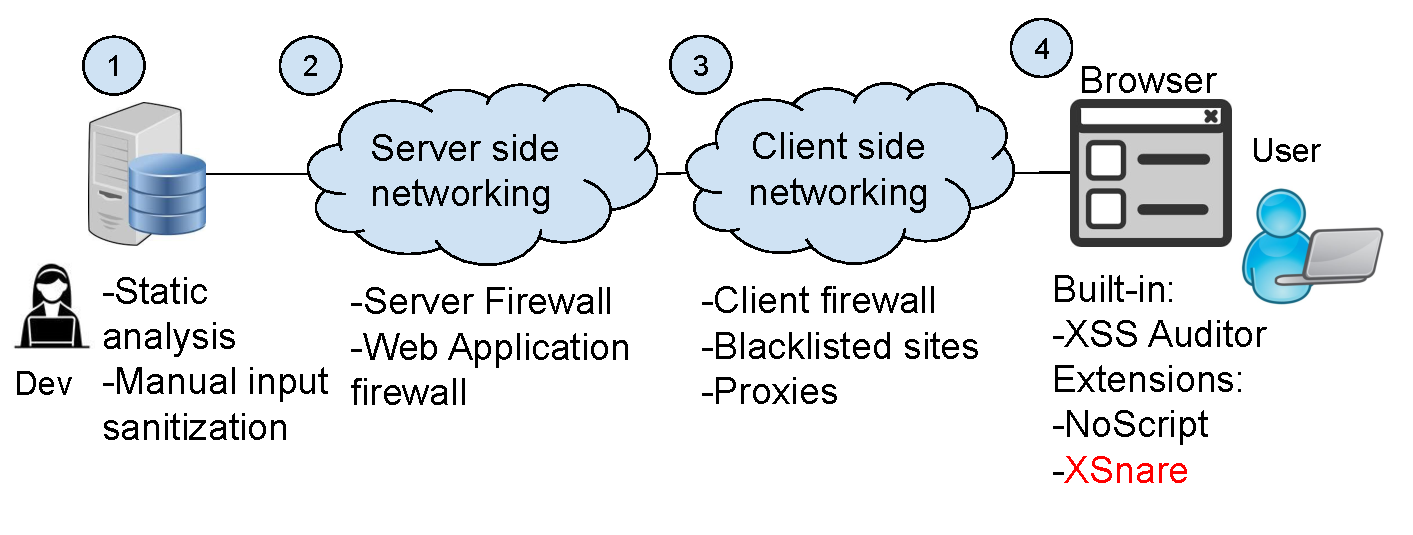
\includegraphics[scale=0.37]{img/web_app_architecture_one.pdf}
  \vspace*{-5.0ex}
  \caption{Architecture of typical web applications. Different security solutions apply at distinct layers.}
  \label{fig:web_architecture}
\end{figure}

Vulnerability defences can be implemented in multiple layers of the web application stack (Figure~\ref{fig:web_architecture}). Each layer opens different defence options:
%Further details of these different approaches are described in Section 5:
\begin{enumerate}
	\item At the application's server-side, the developer is
          trying to defend herself against malicious users. The first
          line of defence from these vulnerabilities lies in the
          application logic itself. The developer might choose to
          ensure safety of the code, either by using third-party
          solutions, or by securing the code themselves, for example,
          by applying static analysis on the server code to detect
          unsanitised input.
	\item In the hosting environment, developers deploy
          defences including generic firewalls and more specific \acp{WAF}, which defend against attacks
          such as \ac{DDoS}, \ac{SQL} injections and \ac{XSS}.
	\item In the client's environment, the user requires protection from
          malicious websites, and may install their own network firewall,
          network filters, and web proxies.
	\item The last line of defence is the browser. \sys operates at this point.
          The browser has built-in defences, such as
          Chrome's \ac{XSS} Auditor~\cite{xssauditor}. But the user can also
          install browser extensions to block malicious requests and
          responses. % such as the NoScript~\cite{Noscript} extension.
\end{enumerate}

Many of these approaches are either unfit for widespread deployment or
do not benefit from an application's contextual knowledge. For
example, a \ac{WAF} might be enough to defend against most \ac{XSS} attacks on
one deployment, but it would require each individual developer to have
the necessary knowledge and resources to integrate one. A network
proxy at the client-side will usually have a generic set of rules to
apply on incoming network traffic, and this will often lead to an
elevated rate of false positives. Browser built-in defences are very
coarse, and will only work on a subset of exploits. Chrome's XSS
Auditor, for example, only attempts to defend against reflected
\ac{XSS}. In fact, Google has recently announced its intention to deprecate
XSS Auditor, with reasons including "Bypasses abound", "It prevents
some legit sites from working", and "Once detected, there’s nothing
good to do"~\cite{deprecatexssauditor}. Stock et
al.~\cite{Stock:2017:WTI:3241189.3241265} propose enhancements to the
XSS Auditor. Their work covers a wider range of exploits than the
auditor, but is limited to DOM-based \ac{XSS}. Our work is not particular
to a type of \ac{XSS}.

While there is much work in the server-side area,
\cite{Xu:2006:TPE:1267336.1267345,DBLP:conf/sec/Nguyen-TuongGGSE05,Pietraszek:2005:DAI:2146257.2146267,Bisht:2008:XPD:1428322.1428325}
(TODO: references for static analysis of php code for security), the
adoption of server-side techniques might not be feasible for many
developers. A 2018 study found that the average time to patch a \ac{CVE}
regardless of severity is 38 days, increasing to as much as 54 days
for low severity vulnerabilities, and the oldest unpatched \ac{CVE} was 340
days old~\cite{Rapid7}. A client-side solution does not rely on
application developers, so it ideally reduces the turnaround time
between a vulnerability and its patch. Furthermore, it is
complementary to the aforementioned techniques: a \ac{WAF} will not reduce
the security of a client-side approach by any means, and having these
two work in tandem is beneficial to the user's experience.

To provide users with the means to protect themselves in the absence
of control over servers, we strongly believe a novel client-side
solution must be delivered. A number of existing solutions in this
area also suffer from a high rate of false-positives and
false-negatives, due to the lack of information available at the
layers they operate at. For example, NoScript works via domain
whitelisting, thus by default, JavaScript scripts and other code will
not execute. However, not all scripts outside of the whitelist should
be assumed to be malicious. Browser-level filters like XSS Auditor
work based on general policies and can therefore incorrectly sanitize
non-malicious content.

In contrast, we posit that the DOM is the right place to interpose for
the purpose of mitigating against these attacks, since we have the
full picture at that point. While most of the functionality we provide
could be done by a network filter on top of the browser, we require
some additional context to perform effective \ac{XSS} identification. In
particular, when an exploit manifests itself through dynamic
behaviour, like a network request initiated by an user's click, we
require knowledge of the tab which initiated the request to filter the
response. Previous work on client-side solutions has focused on
generic approaches to vulnerability detection
\cite{Kirda:2009:CCS:2639535.2639808,Jim:2007:DSI:1242572.1242654,Hallaraker:2005:DMJ:1078029.1078861}. Our
work is application-specific and can therefore be more precise when
targeting vulnerabilities.

Commonly, bug bounty hunters and penetration testers will scour
websites to find vulnerabilities and alert developers of issues in
these, as well as potential fixes. Developers will then fix the bugs
accordingly so that users are not subject to vulnerabilities. Inspired
by this workflow, we believe this process can be partly automated
using a firewall-based approach, so that users don't have to wait for
developers to update their code.

Our system consists of three main components: a trusted Firefox
extension for interposing between the application and the DOM, a
periodically updated local database which maintains exploit
definitions and descriptions of the vulnerabilities to be targeted by
the extension in the form of signatures, and finally, a declarative
language for describing exploits, expressive enough for an user to be
precise about which parts of the HTML are vulnerable and how to
sanitize them.

We aim to reproduce the developer's intended server-side patch on the
client-side, therefore, we need to be able to determine the separation
between dynamic content and the static template, and pass the dynamic
elements to a sanitization function. We provide further details of the
mechanisms we provide to achieve this goal in Section
\ref{xsnare_design}.

We evaluate our application-specific, signature-based approach, by
testing it against recent \ac{XSS} CVEs. CVE databases are well-maintained
and widely available. They are one of the main tools used by
developers to patch their code against known vulnerabilities. To the
best of our knowledge, our work is the first to evaluate an \ac{XSS}
protection tool against real world exploits of this form at the scope
we do.


